\section{Spark::Sp\-Matrix3$<$ Real $>$ Class Template Reference}
\label{classSpark_1_1SpMatrix3}\index{Spark::SpMatrix3@{Spark::SpMatrix3}}
{\tt \#include $<$Sp\-Matrix.h$>$}

Inheritance diagram for Spark::Sp\-Matrix3$<$ Real $>$:\begin{figure}[H]
\begin{center}
\leavevmode
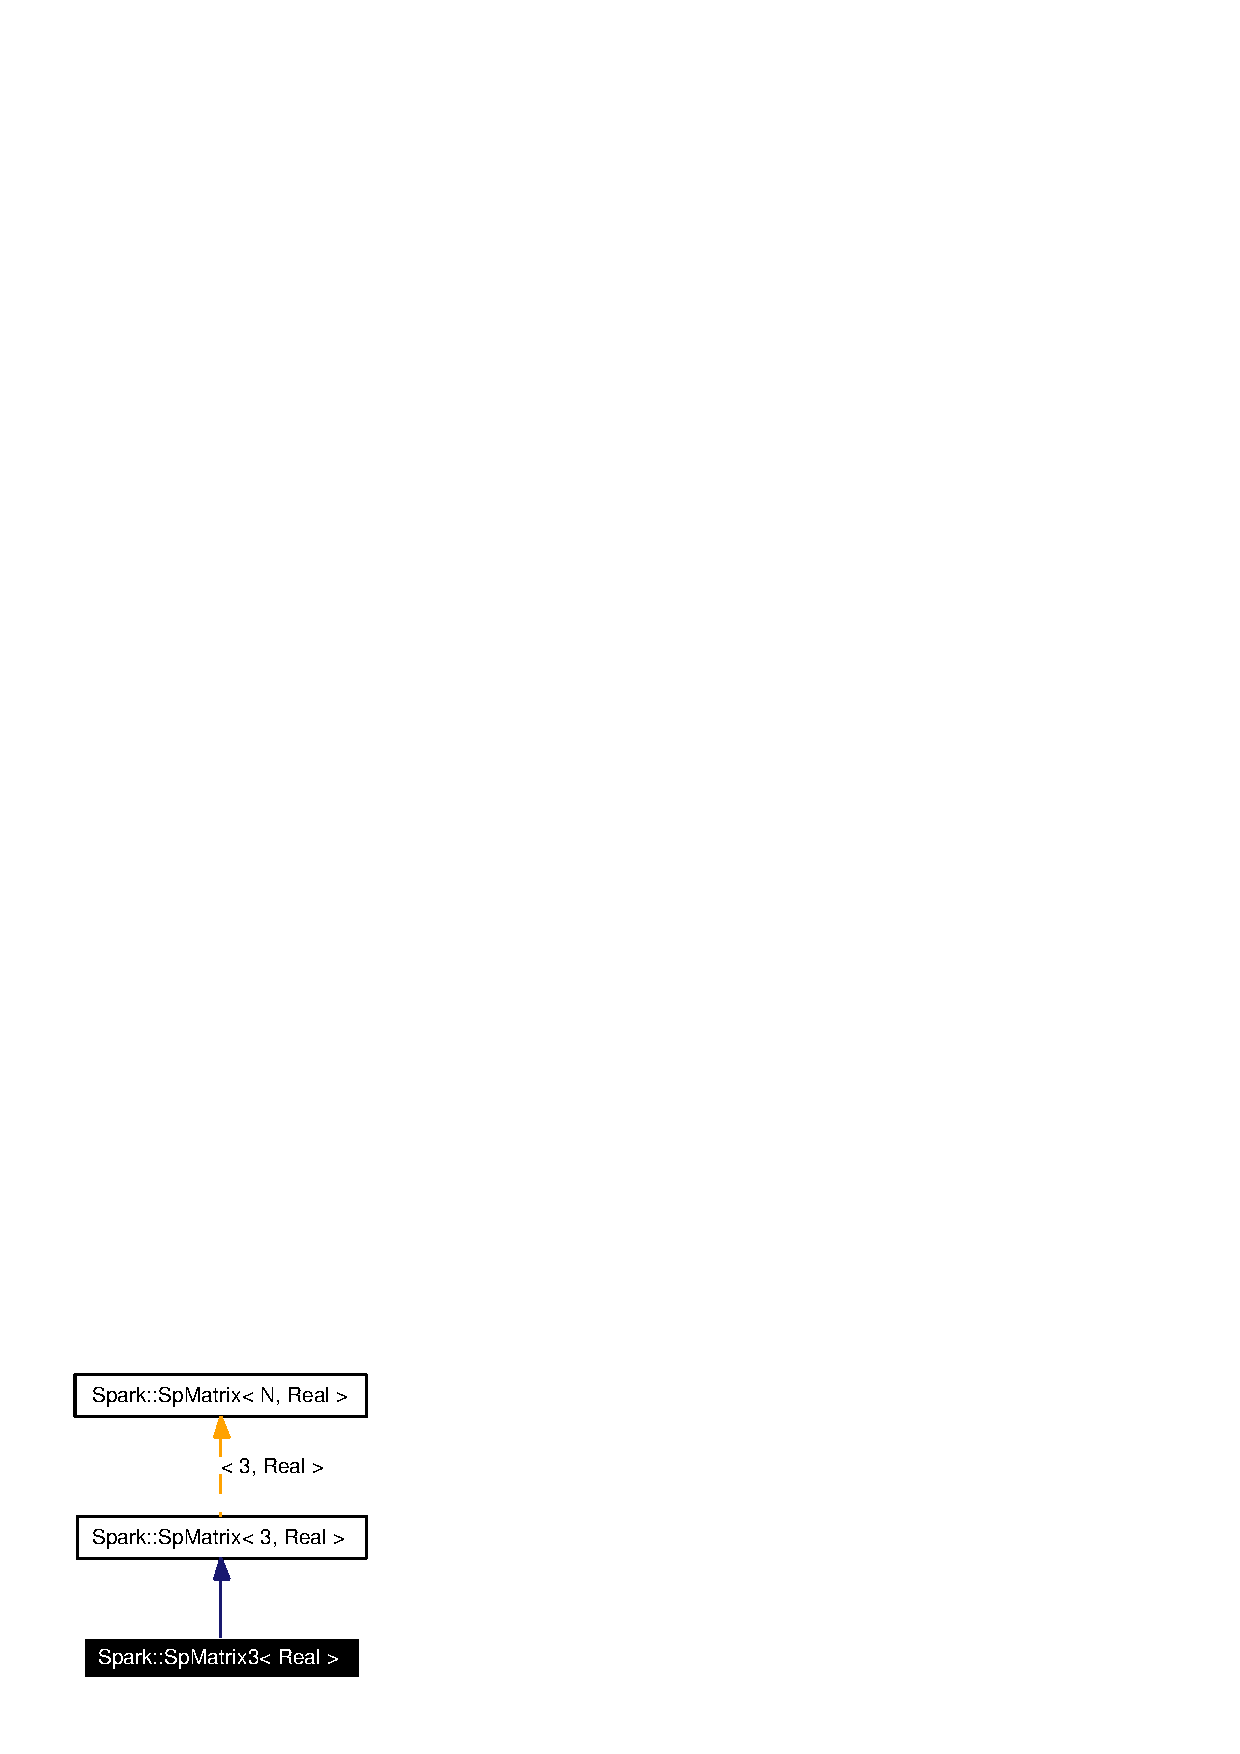
\includegraphics[width=88pt]{classSpark_1_1SpMatrix3__inherit__graph}
\end{center}
\end{figure}
Collaboration diagram for Spark::Sp\-Matrix3$<$ Real $>$:\begin{figure}[H]
\begin{center}
\leavevmode
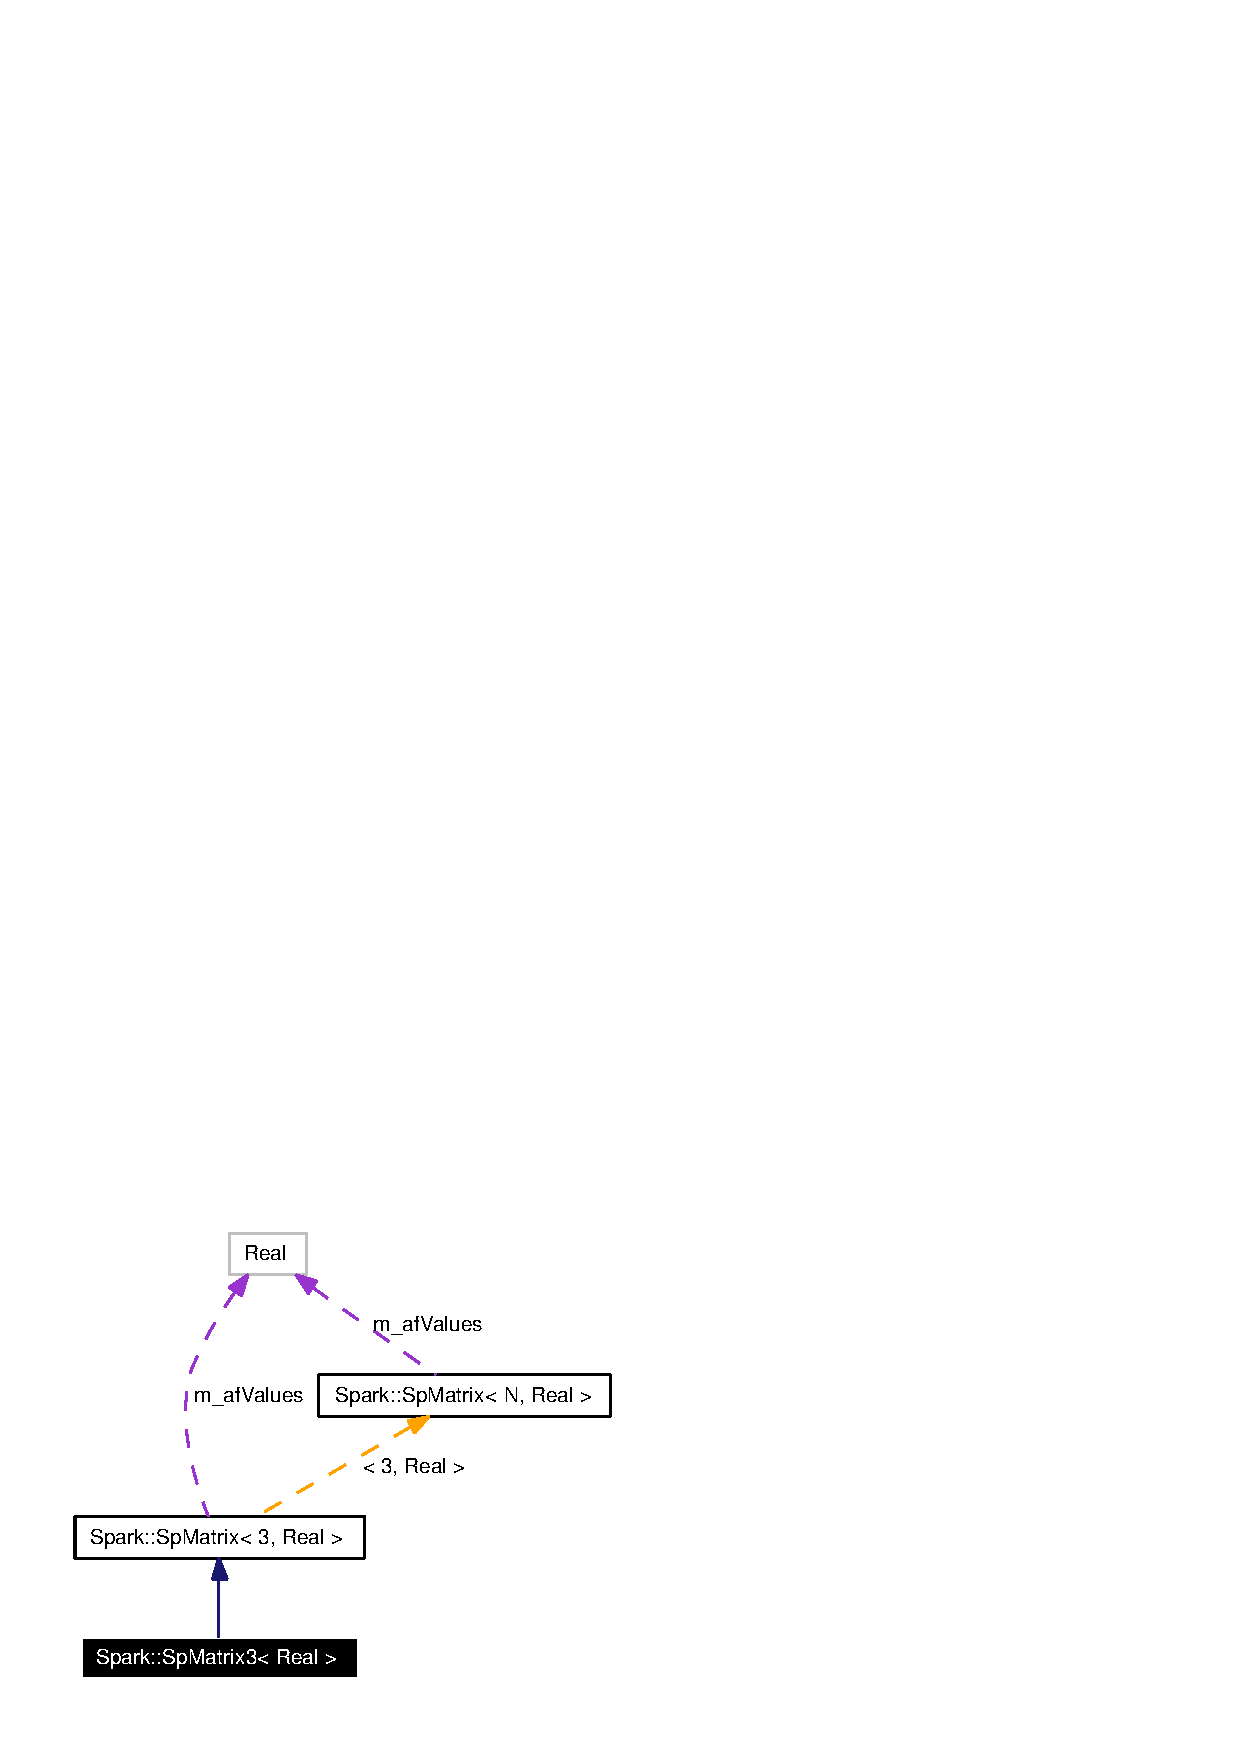
\includegraphics[width=147pt]{classSpark_1_1SpMatrix3__coll__graph}
\end{center}
\end{figure}


\subsection{Detailed Description}
\subsubsection*{template$<$class Real$>$ class Spark::Sp\-Matrix3$<$ Real $>$}

3x3 Matrix class for vector algebra 

Definition at line 134 of file Sp\-Matrix.h.\subsection*{Public Member Functions}
\begin{CompactItemize}
\item 
{\bf Sp\-Matrix3} ()
\item 
{\bf Sp\-Matrix3} (const {\bf Sp\-Matrix3} \&rk\-M)
\item 
{\bf Sp\-Matrix3} (const {\bf Sp\-Matrix}$<$ 3, Real $>$ \&rk\-M)
\item 
{\bf Sp\-Matrix3} (Real f\-M00, Real f\-M01, Real f\-M02, Real f\-M10, Real f\-M11, Real f\-M12, Real f\-M20, Real f\-M21, Real f\-M22)
\item 
{\bf Sp\-Matrix3} (const Real af\-Entry[9], bool b\-Row\-Major)
\item 
{\bf Sp\-Matrix3} (const {\bf Sp\-Tuple3}$<$ Real $>$ \&rk\-U, const {\bf Sp\-Tuple3}$<$ Real $>$ \&rk\-V, const {\bf Sp\-Tuple3}$<$ Real $>$ \&rk\-W, bool b\-Columns)
\item 
{\bf Sp\-Matrix3} (const {\bf Sp\-Tuple3}$<$ Real $>$ $\ast$ak\-V, bool b\-Columns)
\item 
{\bf Sp\-Matrix3} (const {\bf Sp\-Tuple3}$<$ Real $>$ \&rk\-Axis, Real f\-Angle)
\item 
void {\bf From\-Axis\-Angle} (const {\bf Sp\-Tuple3}$<$ Real $>$ \&rk\-Axis, Real f\-Angle)
\item 
{\bf Sp\-Matrix3} \& {\bf operator=} (const {\bf Sp\-Matrix3} \&rk\-M)
\item 
{\bf Sp\-Matrix3} \& {\bf operator=} (const {\bf Sp\-Matrix}$<$ 3, Real $>$ \&rk\-M)
\end{CompactItemize}


\subsection{Constructor \& Destructor Documentation}
\index{Spark::SpMatrix3@{Spark::Sp\-Matrix3}!SpMatrix3@{SpMatrix3}}
\index{SpMatrix3@{SpMatrix3}!Spark::SpMatrix3@{Spark::Sp\-Matrix3}}
\subsubsection{\setlength{\rightskip}{0pt plus 5cm}template$<$class Real$>$ {\bf Spark::Sp\-Matrix3}$<$ Real $>$::{\bf Sp\-Matrix3} ()}\label{classSpark_1_1SpMatrix3_a0}


\index{Spark::SpMatrix3@{Spark::Sp\-Matrix3}!SpMatrix3@{SpMatrix3}}
\index{SpMatrix3@{SpMatrix3}!Spark::SpMatrix3@{Spark::Sp\-Matrix3}}
\subsubsection{\setlength{\rightskip}{0pt plus 5cm}template$<$class Real$>$ {\bf Spark::Sp\-Matrix3}$<$ Real $>$::{\bf Sp\-Matrix3} (const {\bf Sp\-Matrix3}$<$ Real $>$ \& {\em rk\-M})}\label{classSpark_1_1SpMatrix3_a1}


\index{Spark::SpMatrix3@{Spark::Sp\-Matrix3}!SpMatrix3@{SpMatrix3}}
\index{SpMatrix3@{SpMatrix3}!Spark::SpMatrix3@{Spark::Sp\-Matrix3}}
\subsubsection{\setlength{\rightskip}{0pt plus 5cm}template$<$class Real$>$ {\bf Spark::Sp\-Matrix3}$<$ Real $>$::{\bf Sp\-Matrix3} (const {\bf Sp\-Matrix}$<$ 3, Real $>$ \& {\em rk\-M})}\label{classSpark_1_1SpMatrix3_a2}


\index{Spark::SpMatrix3@{Spark::Sp\-Matrix3}!SpMatrix3@{SpMatrix3}}
\index{SpMatrix3@{SpMatrix3}!Spark::SpMatrix3@{Spark::Sp\-Matrix3}}
\subsubsection{\setlength{\rightskip}{0pt plus 5cm}template$<$class Real$>$ {\bf Spark::Sp\-Matrix3}$<$ Real $>$::{\bf Sp\-Matrix3} (Real {\em f\-M00}, Real {\em f\-M01}, Real {\em f\-M02}, Real {\em f\-M10}, Real {\em f\-M11}, Real {\em f\-M12}, Real {\em f\-M20}, Real {\em f\-M21}, Real {\em f\-M22})}\label{classSpark_1_1SpMatrix3_a3}


\index{Spark::SpMatrix3@{Spark::Sp\-Matrix3}!SpMatrix3@{SpMatrix3}}
\index{SpMatrix3@{SpMatrix3}!Spark::SpMatrix3@{Spark::Sp\-Matrix3}}
\subsubsection{\setlength{\rightskip}{0pt plus 5cm}template$<$class Real$>$ {\bf Spark::Sp\-Matrix3}$<$ Real $>$::{\bf Sp\-Matrix3} (const Real {\em af\-Entry}[9], bool {\em b\-Row\-Major})}\label{classSpark_1_1SpMatrix3_a4}


\index{Spark::SpMatrix3@{Spark::Sp\-Matrix3}!SpMatrix3@{SpMatrix3}}
\index{SpMatrix3@{SpMatrix3}!Spark::SpMatrix3@{Spark::Sp\-Matrix3}}
\subsubsection{\setlength{\rightskip}{0pt plus 5cm}template$<$class Real$>$ {\bf Spark::Sp\-Matrix3}$<$ Real $>$::{\bf Sp\-Matrix3} (const {\bf Sp\-Tuple3}$<$ Real $>$ \& {\em rk\-U}, const {\bf Sp\-Tuple3}$<$ Real $>$ \& {\em rk\-V}, const {\bf Sp\-Tuple3}$<$ Real $>$ \& {\em rk\-W}, bool {\em b\-Columns})}\label{classSpark_1_1SpMatrix3_a5}


\index{Spark::SpMatrix3@{Spark::Sp\-Matrix3}!SpMatrix3@{SpMatrix3}}
\index{SpMatrix3@{SpMatrix3}!Spark::SpMatrix3@{Spark::Sp\-Matrix3}}
\subsubsection{\setlength{\rightskip}{0pt plus 5cm}template$<$class Real$>$ {\bf Spark::Sp\-Matrix3}$<$ Real $>$::{\bf Sp\-Matrix3} (const {\bf Sp\-Tuple3}$<$ Real $>$ $\ast$ {\em ak\-V}, bool {\em b\-Columns})}\label{classSpark_1_1SpMatrix3_a6}


\index{Spark::SpMatrix3@{Spark::Sp\-Matrix3}!SpMatrix3@{SpMatrix3}}
\index{SpMatrix3@{SpMatrix3}!Spark::SpMatrix3@{Spark::Sp\-Matrix3}}
\subsubsection{\setlength{\rightskip}{0pt plus 5cm}template$<$class Real$>$ {\bf Spark::Sp\-Matrix3}$<$ Real $>$::{\bf Sp\-Matrix3} (const {\bf Sp\-Tuple3}$<$ Real $>$ \& {\em rk\-Axis}, Real {\em f\-Angle})}\label{classSpark_1_1SpMatrix3_a7}




\subsection{Member Function Documentation}
\index{Spark::SpMatrix3@{Spark::Sp\-Matrix3}!FromAxisAngle@{FromAxisAngle}}
\index{FromAxisAngle@{FromAxisAngle}!Spark::SpMatrix3@{Spark::Sp\-Matrix3}}
\subsubsection{\setlength{\rightskip}{0pt plus 5cm}template$<$class Real$>$ void {\bf Spark::Sp\-Matrix3}$<$ Real $>$::From\-Axis\-Angle (const {\bf Sp\-Tuple3}$<$ Real $>$ \& {\em rk\-Axis}, Real {\em f\-Angle})}\label{classSpark_1_1SpMatrix3_a8}


\index{Spark::SpMatrix3@{Spark::Sp\-Matrix3}!operator=@{operator=}}
\index{operator=@{operator=}!Spark::SpMatrix3@{Spark::Sp\-Matrix3}}
\subsubsection{\setlength{\rightskip}{0pt plus 5cm}template$<$class Real$>$ {\bf Sp\-Matrix3}\& {\bf Spark::Sp\-Matrix3}$<$ Real $>$::operator= (const {\bf Sp\-Matrix}$<$ 3, Real $>$ \& {\em rk\-M})}\label{classSpark_1_1SpMatrix3_a10}


\index{Spark::SpMatrix3@{Spark::Sp\-Matrix3}!operator=@{operator=}}
\index{operator=@{operator=}!Spark::SpMatrix3@{Spark::Sp\-Matrix3}}
\subsubsection{\setlength{\rightskip}{0pt plus 5cm}template$<$class Real$>$ {\bf Sp\-Matrix3}\& {\bf Spark::Sp\-Matrix3}$<$ Real $>$::operator= (const {\bf Sp\-Matrix3}$<$ Real $>$ \& {\em rk\-M})}\label{classSpark_1_1SpMatrix3_a9}




The documentation for this class was generated from the following file:\begin{CompactItemize}
\item 
{\bf Sp\-Matrix.h}\end{CompactItemize}
